%\documentclass[9pt]{elife}
\documentclass[multi=figure,9pt]{standalone}
\usepackage{graphicx}

\RequirePackage[T1]{fontenc}
\RequirePackage[utf8]{inputenc}
\RequirePackage{stix}
\RequirePackage[default]{opensans}
\renewcommand{\ttdefault}{lmtt}

\RequirePackage{microtype}

% Trueno/Open Sans requires a bigger "single" linespread.
\linespread{1.2}
\if@onehalfspacing\linespread{1.5}\fi
\if@doublespacing\linespread{2.0}\fi

\RequirePackage{graphicx,xcolor}
\definecolor{eLifeDarkBlue}{HTML}{273B81}
\definecolor{eLifeLightBlue}{HTML}{0A9DD9}
\definecolor{eLifeMediumGrey}{HTML}{6D6E70}
\definecolor{eLifeLightGrey}{HTML}{929497}

\RequirePackage{booktabs}
\RequirePackage{authblk}

\RequirePackage{changepage}

\RequirePackage{silence}
\WarningFilter{caption}{The option `hypcap=true' will be ignored}

\RequirePackage[labelfont={bf},%
                labelsep=period,%
                justification=raggedright,%
                singlelinecheck=true,%
                tableposition=top,font={color=eLifeDarkBlue,scriptsize}]
                {caption}

\makeatletter
\renewenvironment{figure}%
{\def\@captype{figure}%
\minipage{\textwidth}}%
{\endminipage}
\makeatother

\let\efloatseparator=\empty

\usepackage{subcaption}

\begin{document}

\begin{figure}
    \centering
    \captionsetup[subfigure]{font={color=eLifeDarkBlue,footnotesize}}
    \subcaptionbox{The structure element.}{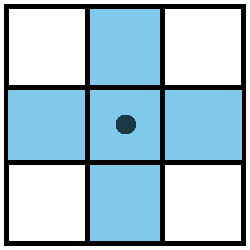
\includegraphics[width=0.25\textwidth]{structure.pdf}}
    \subcaptionbox{The original image.}{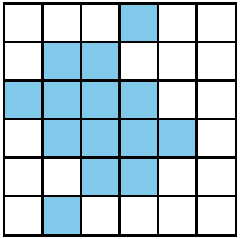
\includegraphics{structure_image_before.pdf}}
    \subcaptionbox{Image modified by the structure element.}{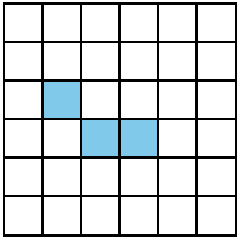
\includegraphics{structure_image_after.pdf}}
    % \begin{subfigure}[b]{0.25\textwidth}
    %         \centering
    %        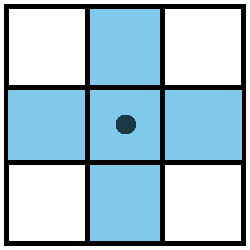
\includegraphics[width=\textwidth]{structure}
    %         \caption{The structure element.}
    %         \label{fig:b}
    % \end{subfigure}
    % \begin{subfigure}[b]{0.36\textwidth}
    %        \centering
    %         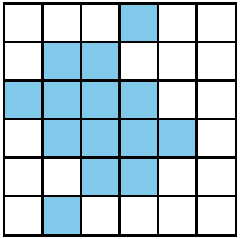
\includegraphics[width=\textwidth]{structure_image_before}
    %         \caption{The original image.}
    %         \label{fig:a}
    % \end{subfigure}
    % \begin{subfigure}[b]{0.36\textwidth}
    %         \centering
    %         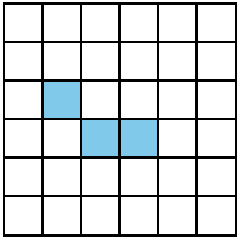
\includegraphics[width=\textwidth]{structure_image_after}
    %         \caption{Image modified by the structure element.}
    %         \label{fig:c}
    % \end{subfigure}
\end{figure}

\end{document}